\appendix

\section{Analysis of the dataset with air speed measurements at three heights}\label{sec:analysis-of-the-dataset-with-air-speed-measurements-at-three-heights}

In this section, we analyzed the dataset with air speed measurements at three heights.
Only eight papers in the \ac{db2} had air speed measurements at three heights with \ac{v}~$\geq$~\qty{0.2}{\m\per\s}.
A summary of the papers is provided in Table~\ref{tab:three_heights_papers}.
The table also shows the number of measurements for each paper and how much (percentage) each study contributed to the dataset.
\begin{table}[htb!]
    \centering
    \begin{tabular}{lrr}
\toprule
Publication & Count & \% Total \\
\midrule
Cena, K., and de Dear, R. J. (1999) & 827 & 27 \\
de Dear, R.J. and Fountain, M.E. (1994) & 704 & 23 \\
Zhang, Y., Chen, H., Meng, Q. (2013) & 465 & 15 \\
Zhang, Y. et al. (2010) & 416 & 14 \\
Schiller (Brager), G. (1990) & 304 & 10 \\
Donnini, G. et al. (1996) & 192 & 6 \\
Tartarini, F., Cooper, P., Fleming, R. (2018) & 113 & 4 \\
Benton, C. C. and Brager, G. S. (1994) & 30 & 1 \\
\bottomrule
\end{tabular}

    \caption{F1-score for the \ac{pmv} and \ac{pmv-ce} models for different subsets of data.}
    \label{tab:three_heights_papers}
\end{table}
The paper by Zhang et al.\ and Cena et al.\ contributed the most to the dataset with \qty{58}{\percent} and \qty{23}{\percent}, respectively.
These \num{1184} where used to compare the \ac{pmv} and \ac{pmv-ce} models using the same methodology as in Section~\ref{sec:results}.
The air speed distribution at the three heights for each paper is shown in Figure~\ref{fig:boxenplot_wind_speed_three_heights}.
\begin{figure}[htb!]
    \centering
    
\includegraphics[width=\textwidth]{figures/boxenplot_wind_speed_three_heights}
    \caption{Wind speeds distribution at three heights.}
    \label{fig:boxenplot_wind_speed_three_heights}
\end{figure}
The distribution of air speed at the three heights varies between the papers, hence, it is difficult to make generalizations.
However, it should be noted that in most of the studies the air speed measured at the chest height was a good representation of the air speed at the other two heights.
This assumption is not valid for Brenton et al.\ (1994) and Donnini et al.\ (1996) it should be noted that these two studies had a only \num{11} and \num{7} measurements, respectively.
In this section we are not showing the F1-score for the \ac{pmv} and \ac{pmv-ce} models for the different subsets of data since we have already presented the results in Table~\ref{tab:f1}.
We would like to remind the reader that the F1-score for \ac{pmv-ce} model was lower than the \ac{pmv} model for this subset of data, i.e, \ac{v}~$\geq$~\qty{0.2}{\m\per\s} and \ac{v} measured at three heights.
As previously discussed this is an unexpected result since the \ac{pmv} should be significantly more accurate than the \ac{pmv-ce} model for this subset of data.
In this section we are not showing the accuracy of the \ac{pmv} and \ac{pmv-ce} model as a function of the \ac{tsv} since we have a very limited number of measurements for this subset of data moreover this analysis has some limitations as previously discussed.

We, however, plotted the \ac{pmv} and \ac{pmv-ce} values against the \ac{tsv} values and we plotted the \ac{lowess} curves to visualize the prevailing data trend.
The results are shown in Figure~\ref{fig:bubble_models_vs_tsv_three_heights}.
\begin{figure*}[htb!]
    \centering
    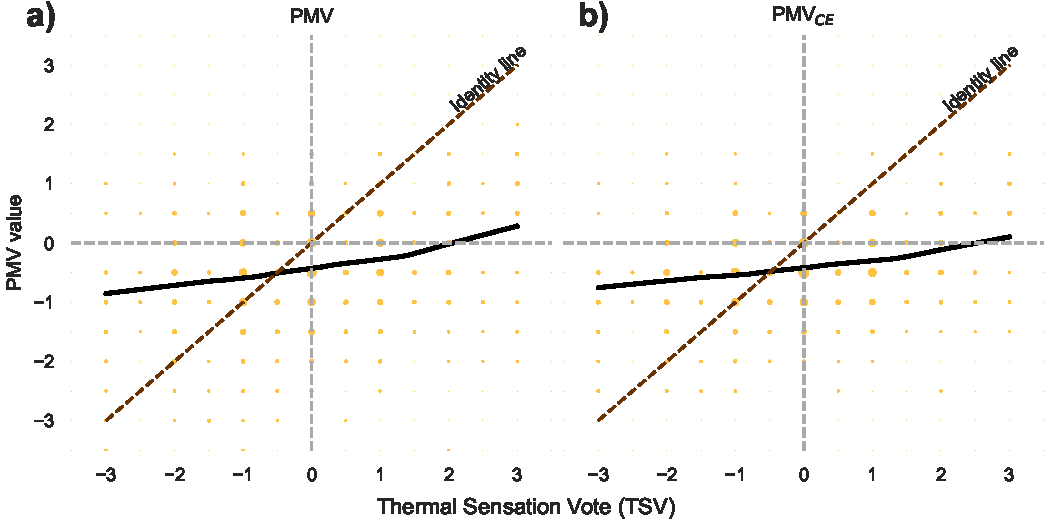
\includegraphics[width=\textwidth]{figures/bubble_models_vs_tsv_three_heights}
    \caption{The \ac{lowess} curve shows the relationship between the raw \ac{pmv} and \ac{tsv} data for the dataset with \ac{v}~$\geq$~\qty{0.2}{\m\per\s} and measured at three heights.
    Raw data were then binned and a bubble chart (circle area is proportional to the number of votes in that bin) was superimposed over the regression curve to aid the visualization of a large dataset.
    The brown dashed line represents the identity line where the slope is 1 and the intercept is 0.
    Comparison between the \ac{pmv} and \ac{pmv-ce} models for the dataset with air speed measured at three heights.}
    \label{fig:bubble_models_vs_tsv_three_heights}
\end{figure*}
The results show that the \ac{pmv} model is more accurate than the \ac{pmv-ce} model.
The intercept of the \ac{pmv} model is \num{-.2} while the intercept of the \ac{pmv-ce} model is \num{-.39}.
Moreover, the \ac{pmv-ce} \ac{lowess} curve is only marginally higher than \num{0} despite partcipants reporting a \ac{tsv} of \num{3}.

Despite the fact that these results already showing that the \ac{pmv} model is more accurate than the \ac{pmv-ce} model for this subset of data, we also calculated the overall bias of the \ac{pmv} and \ac{pmv-ce} models.
The results are shown in Figure~\ref{fig:hist_discrepancies_three_heights}.
\begin{figure}[htb!]
    \centering
    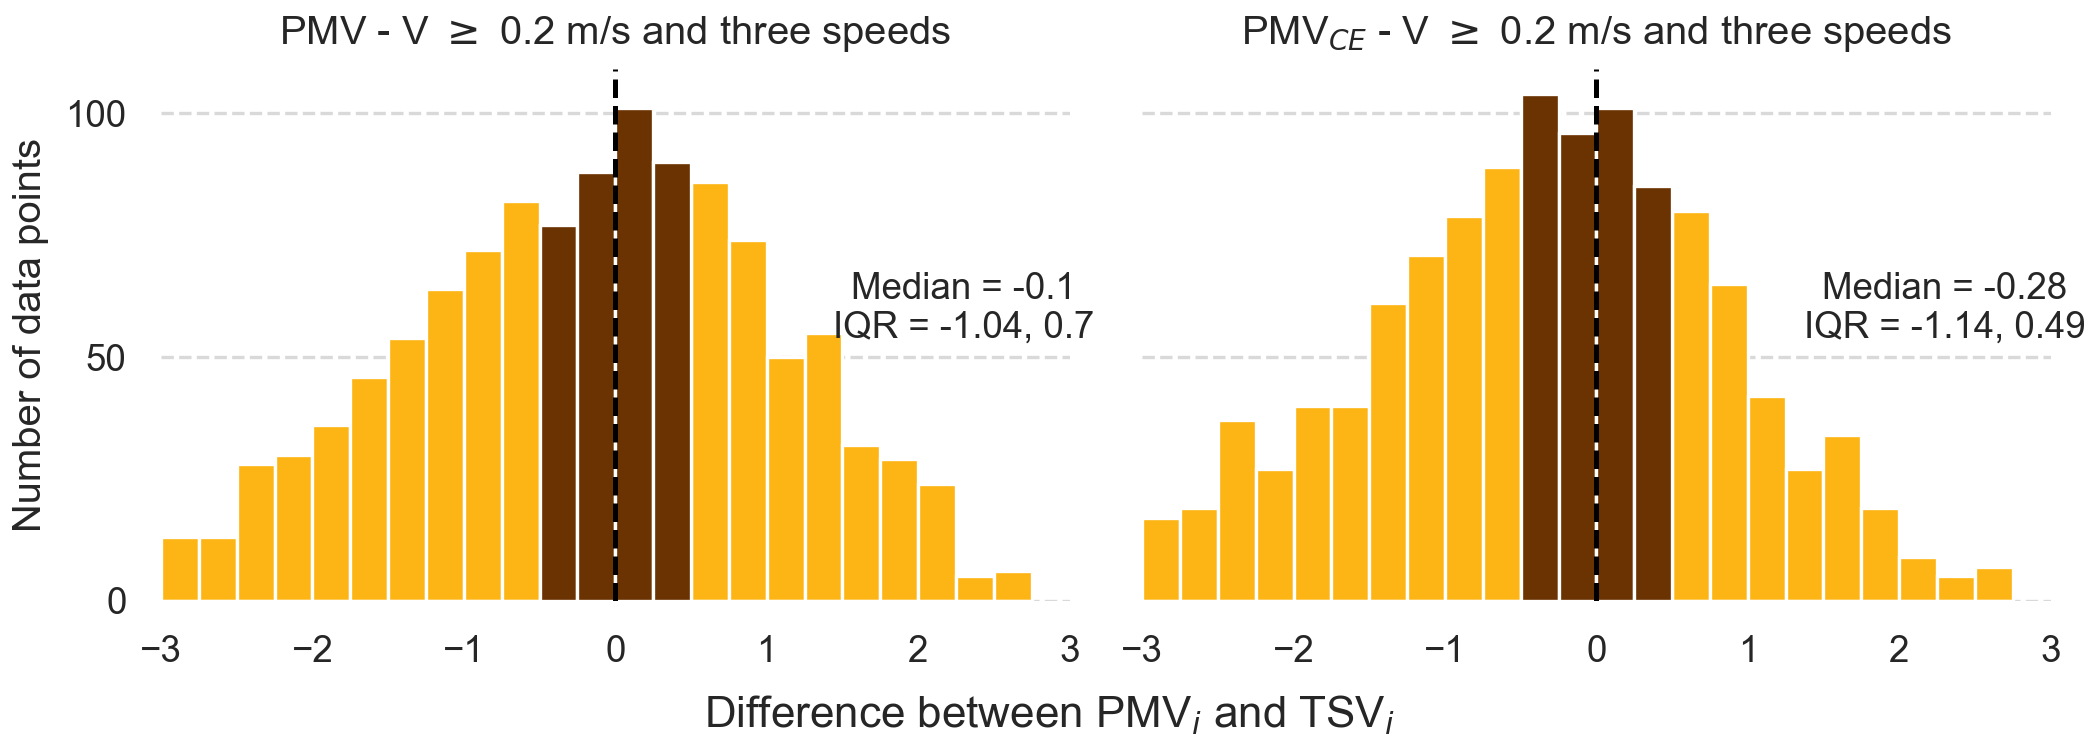
\includegraphics[width=\textwidth]{figures/hist_discrepancies_three_heights}
    \caption{Bias of the \ac{pmv} and \ac{pmv-ce} models for the dataset with air speed measured at three heights.}
    \label{fig:hist_discrepancies_three_heights}
\end{figure}
The \ac{pmv} model has a bias of \num{-.1} while the \ac{pmv-ce} model has a bias of \num{-.28}.
Moreover, the distribution of the discrepancies for the \ac{pmv} model is more centered around \num{0} than the \ac{pmv-ce} model.
These results allows us to conclude that the \ac{pmv} model is more accurate than the \ac{pmv-ce} model for the dataset with air speed measured at three heights.
Consequently, we recommend using the \ac{pmv} model instead of the \ac{pmv-ce}.

%\section{Comparison between the PMV formulations with the \ac{pmvg}}\label{sec:comparison-between-the-pmv-formulations-with-the-two-node-model}
%We compared how the results of the \ac{pmv} and \ac{pmv-ce} perform against the results of the \ac{pmvg}.
%% SS provide more information why this was done
%% Stefano Schiavon: Please provide more details of how these inputs were generated, within which ranges, etc.
%Figure~\ref{fig:pmv_two_node_comparison} was generated by calculating the three \ac{pmv} values using the same combination of \num{10000} randomly generated sets inputs.
%The \ac{pmv} and \ac{pmv-ce} were then plotted on the y-axis while the \ac{pmvg} value was on the x-axis.
%The Figure also shows the \ac{lowess} curves that are used to visualize the prevailing data trend.
%% Stefano Schiavon: Beside the visualization, can you discuss here also the quantitative results to support the conclusion?
%The results of the \ac{pmv} model had a higher agreement than those obtained with the \ac{pmv-ce} model for \ac{pmvg} $\geq$ \qty{0.5}{\m\per\s}.
%% Stefano Schiavon: This is unclear and cannot be deduced from the figure, from where does it come from? How can a PMV model be described by an air speed?
%These results show the \ac{pmv-ce} is less similar to the \ac{pmvg} model than the \ac{pmv}, despite using it in the backend to calculate the cooling effect.
%This is also an unexpected result and we will discuss why this may be in the following paragraph.
%% SS When a figure report how well a variable is predicted, for example x-measured vs x-predicted, the graph must be a square, otherwise it is visually skewed. 1) I suggest to use the words instead of numbers for PMV 2) We should be consistent with the PMV naming we used (do not use ASHRAE and ISO here) 3) why both models are far from Gagge for PMV<0, both model in general produce a cooler feeling than PMVgagge, we should explain why if we keep this paper.
%
%\begin{figure*}[htb!]
%    \centering
%    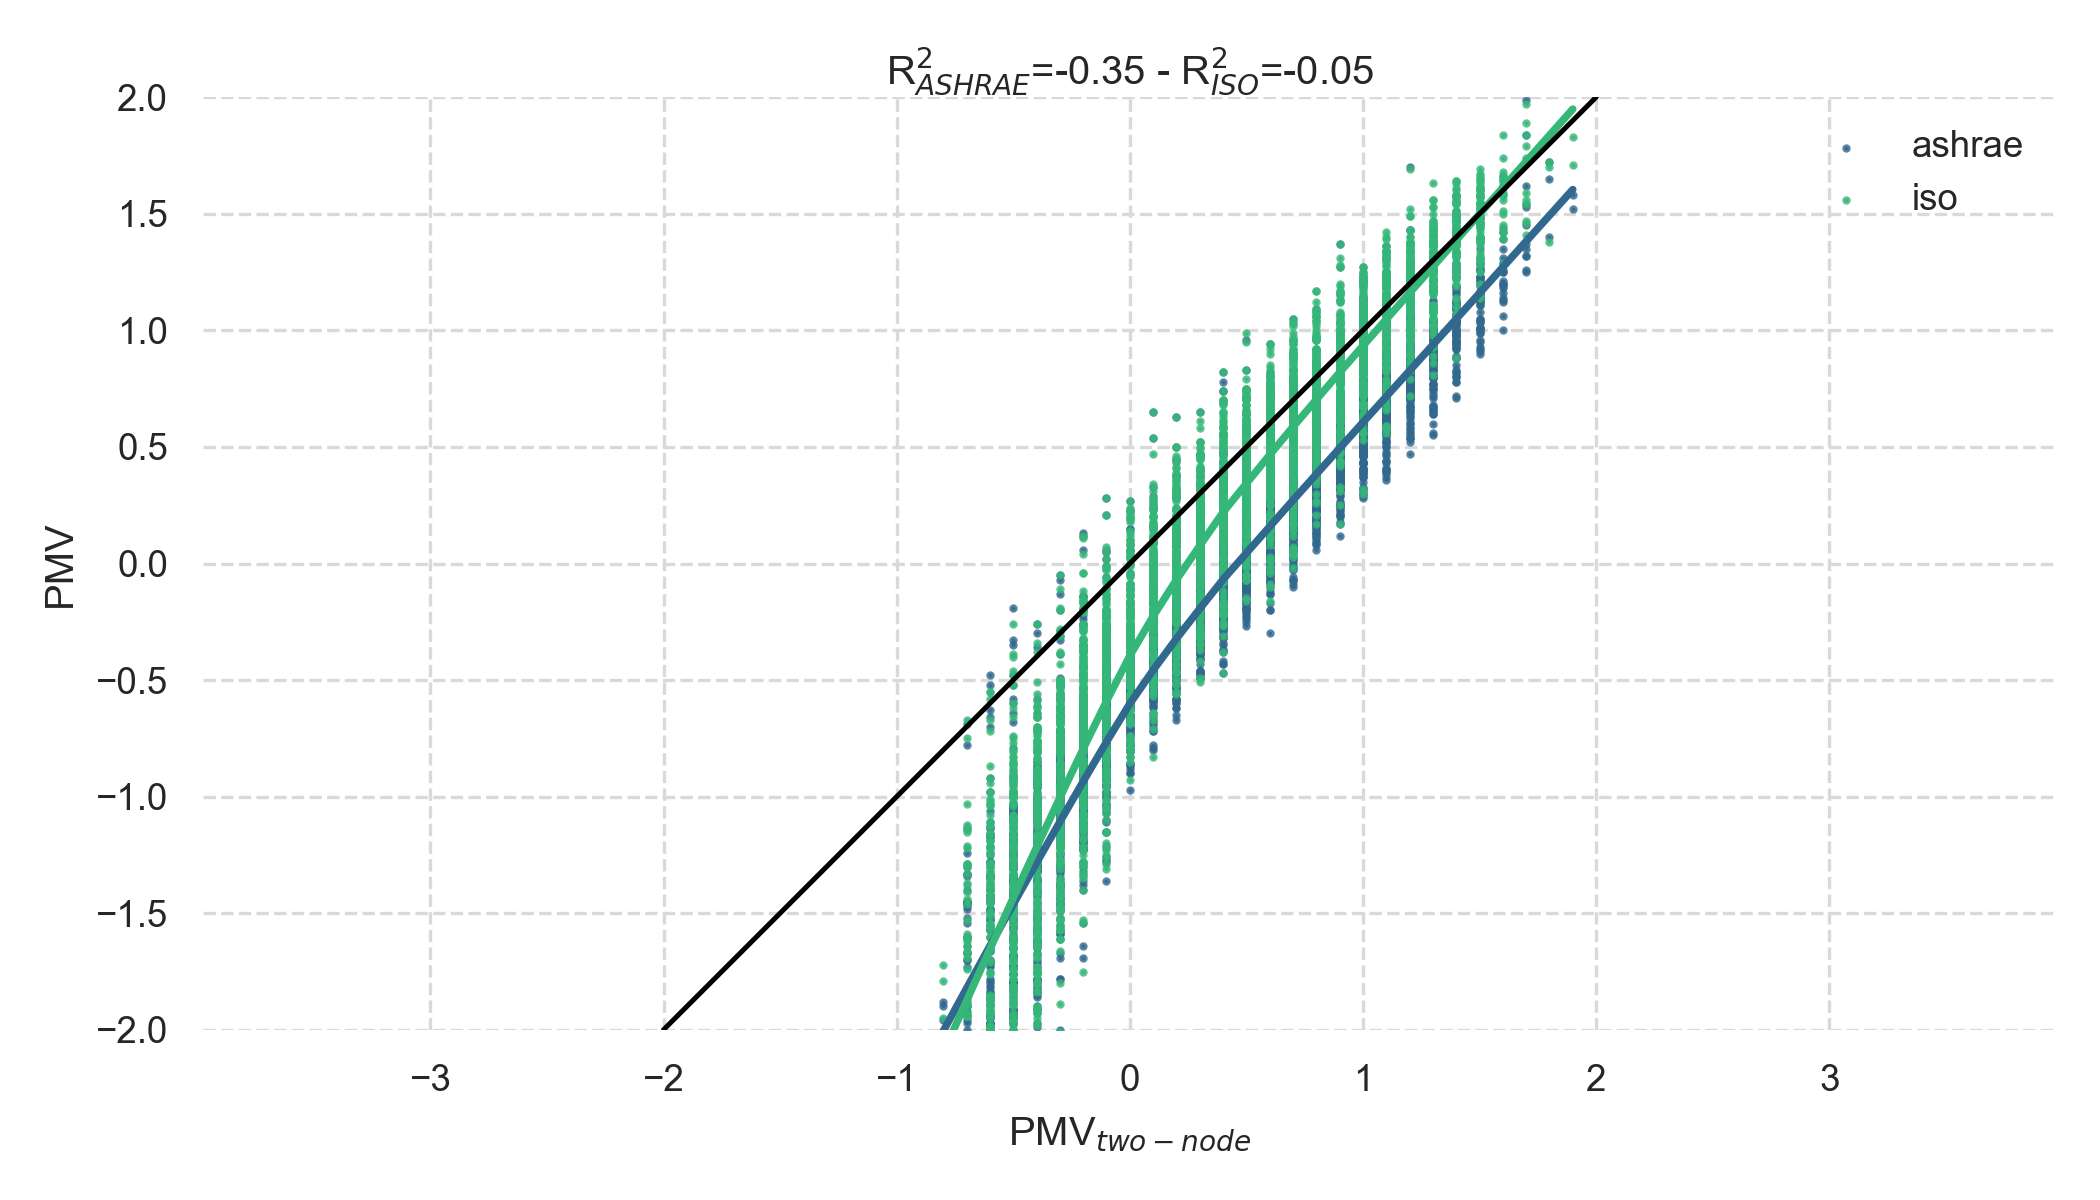
\includegraphics[width=\textwidth]{figures/pmv_two_node_comparison}
%    \caption{}
%    \label{fig:pmv_two_node_comparison}
%\end{figure*}
%
%% todo include the folling
%%I think it is reasonable to have an appendix where we do the analysis for the dataset with only three heights.
%%Given that we have only five authors, we can provide a bit more info about those, maybe in a table format, (paper DOI, publication year, measuring heights, type of anemometer, accuracy, compliance with ISO 7726 or ASHRAE 55, type of building, how long they measure, etc) and have a graph of air speed letter-plot as you did in the email to Ed. For example, for the Yufeng's paper he specified that he followed ISO 7726 (so very good), he used an omni-directional anemometer with a range of 0-5 m/s and accuracy of +-0.02 m/s between 0 and 0.99 m/s and +-0.1 m/s between 1 and 5 m/s). The measurements were taken at 0.1, 0.6 and 1.1 m.